% =====================================================================
% DASFAA 2027 submission -- Springer LNCS, <= 16 pages incl. references.
% Every number in this file is taken from data/*.csv (see scripts/ and the
% comments next to each table). Do not edit numbers by hand.
% =====================================================================
\documentclass[runningheads]{llncs}

\usepackage[T1]{fontenc}
\usepackage{lmodern}
\usepackage{microtype}
\usepackage{graphicx}
\usepackage{booktabs}
\usepackage{array}
\usepackage{xurl}
\usepackage{multirow}
\usepackage{amsmath,amssymb}
\usepackage{xcolor}
\usepackage[pdfauthor={},pdftitle={},hidelinks]{hyperref}

\newcommand{\MV}{\textsc{mv}}
\newcommand{\UV}{\textsc{uv}}
\newcommand{\Ben}{B}
\newcommand{\Rel}{R}
\newcommand{\Sen}{S}
\newcommand{\GC}{\mathrm{GC}}
\newcommand{\tfm}{\mbox{TimesFM-3}}
\setlength{\emergencystretch}{1.5em}
\newcommand{\ci}[2]{\mbox{\scriptsize[$#1$,\,$#2$]}}
\newcommand{\sig}{$^{\ast}$}
\newcommand{\vc}[3]{\begin{tabular}[t]{@{}c@{}}#1\\[-1pt]{\tiny[$#2$,\,$#3$]}\end{tabular}}

\begin{document}

\title{Does Variate Attention Pay Off? Probing Cross-Channel Information Use
in Multivariate Time-Series Foundation Models}
\titlerunning{Probing Cross-Channel Information Use in Multivariate TSFMs}
\author{Anonymous Author(s)}
\authorrunning{Anonymous}
\institute{Anonymous Institution\\\email{anonymous@placeholder.org}}
\maketitle

\begin{abstract}
In multivariate time-series foundation models such as \tfm{}, each channel
attends to the others, and the multivariate mode ranks better on public
benchmarks than univariate forecasting. Whether this gain comes from
information carried by the other channels is untested. We probe \tfm{} within one set of weights: on
identical windows we compare its univariate (\UV) and multivariate (\MV)
modes, corrupt the context channels while leaving the target intact, and
compare the model with Kalman-filter oracles on synthetic systems. On eight
benchmarks the benefit of the \MV{} mode ranges from $-31.95\%$ (Solar-Energy,
$H{=}720$) to $+8.04\%$ (Weather, $H{=}96$). On Electricity, context
channels replaced by week-aligned history keep half of the gain
($\Rel{=}0.50$), whereas unaligned history makes the forecast worse than
using no context ($\Rel{=}2.06$); a one-hour shift is harmless. An injected
leading indicator is exploited, but a synthetic lead--lag driver is not: the
model closes at most 29\% of the oracle gap and gains about 3\% even on
independent channels. Under the reference evaluator, channels outside the
target's block of 32 leave the forecast unchanged while latency grows from
55 to 217\,ms. We derive guidelines for aligning, grouping and gating
channels.
\keywords{Time-series foundation models \and Channel dependence \and
Multivariate forecasting \and Model probing \and Interventions}
\end{abstract}

% =====================================================================
\section{Introduction}\label{sec:intro}

Time-series foundation models (TSFMs) forecast series they were not trained
on~\cite{das2024timesfm,ansari2024chronos,woo2024moirai}. The first
generation treated every channel as a separate univariate series. The
current generation adds attention across channels: \tfm{}~\cite{timesfm3_blog2026}
inserts a variate-attention sublayer into each of its 20 layers,
Chronos-2~\cite{ansari2025chronos2} shares information within groups of
series, and Toto~2.0~\cite{khwaja2026toto2} and TiRex-2~\cite{carlsen2026tirex2}
alternate or restrict attention across variates. These models report better
aggregate ranks on GIFT-Eval~\cite{gifteval2024},
fev-bench~\cite{fevbench2025} and TIME~\cite{timebench2026}.

Other evidence points the other way. Moirai 2.0~\cite{liu2025moirai2} drops
the any-variate attention of its predecessor and forecasts each variate
independently. Liu et al.~\cite{liu2026falconx} observe that Chronos-2
produces almost identical forecasts on GIFT-Eval with and without group
attention. For supervised models, channel independence is hard to
beat~\cite{nie2023patchtst,zeng2023dlinear}; Han et
al.~\cite{han2024capacity} attribute this to robustness under distribution
drift, and Abdelmalak et al.~\cite{abdelmalak2025lookback} show that standard
benchmarks carry weak inter-channel dependence. A higher rank for a
multivariate TSFM is therefore consistent with two explanations: the model
reads predictive information from other channels, or it profits from them in
a way that does not depend on their content.

Leaderboards cannot separate the two, because they compare different models
over heterogeneous tasks. We probe one model from the inside. With the
weights and the target channel fixed, we switch variate attention off and on,
intervene on the context channels, and measure how accuracy and the forecast
itself respond. We ask four questions.
\textbf{RQ1} Where does the \MV{} mode help and where does it hurt?
\textbf{RQ2} Which properties of the context channels does the gain rely on?
\textbf{RQ3} On systems with known cross-channel information, how much of it
does the model extract?
\textbf{RQ4} How many channels, and which ones, should be supplied, and at
what cost?

\noindent Our contributions are:
\begin{itemize}
  \item A within-model probing protocol with four measures (benefit,
        reliance, sensitivity, oracle gap closure), a set of interventions
        with negative and positive controls, and paired bootstrap statistics
        (Sect.~\ref{sec:method}).
  \item Evidence on eight benchmarks and synthetic systems that the \MV{}
        gain of \tfm{} is dataset-specific, depends on calendar-consistent
        and recent context rather than step-level synchrony, and is partly
        independent of cross-channel information (Sect.~\ref{sec:results}).
  \item A cost analysis showing that the reference evaluator isolates
        channels in blocks of 32, so extra channels add latency but no
        information, and a set of data-engineering guidelines derived from
        the measurements (Sect.~\ref{sec:guidelines}).
\end{itemize}

% =====================================================================
\section{Background and Motivation}\label{sec:background}

\subsubsection{\tfm.}
\tfm{} is a 330M-parameter decoder with 20 layers. Each layer applies causal
attention along time with rotary position embeddings, then attention across
variates without position encoding, then a feed-forward block. The input is
split into patches of 32 steps; the forecast horizon is appended as masked
patches and decoded in a single forward pass. Every channel is normalized
from the start of its context. Because variate attention carries no position
information, the model is equivariant to the order of channels, which our
control N1 confirms numerically (Sect.~\ref{sec:rq2}). In the \MV{} mode all
channels in a forward pass are forecast jointly, and each serves both as a
target and as context for the others; past-only covariates are handled in
the same way. In the \UV{} mode each channel is processed alone.

\subsubsection{The 32-variate block.}
The reference evaluator places at most 32 variates in one forward pass. For
a dataset with more channels it forms consecutive blocks of 32 in column
order and pads the last block by repeating channels. Electricity
(321 channels) is thus processed as 11 independent blocks, and a channel
attends only to the 31 other members of its block. ``Multivariate'' results
on high-dimensional data therefore refer to a fixed, order-dependent
grouping, not to attention over all channels. Sect.~\ref{sec:rq4} measures
what this costs and what removing the cap changes.

\subsubsection{Why a within-model probe.}
Comparisons between models confound variate attention with every other
design choice, and attention weights need not explain
predictions~\cite{jain2019attention}. Switching variate attention off inside
one model and manipulating its inputs avoids both problems.

% =====================================================================
\section{Probing Methodology}\label{sec:method}

\subsection{Modes and Measures}
For a test window $w$ and a target channel $i$, the model receives the
target history and the histories of a set $\mathcal{C}_i$ of context
channels and returns a forecast of length $H$. In the \UV{} mode
$\mathcal{C}_i=\emptyset$; in the \MV{} mode $\mathcal{C}_i$ is the block
that contains $i$. An intervention $\pi$ modifies only the channels in
$\mathcal{C}_i$. We write $\hat y^{\UV}_{w,i}$, $\hat y^{\MV}_{w,i}$ and
$\hat y^{\pi}_{w,i}$ for the three forecasts and $e(\cdot)$ for the mean
squared error over the horizon on the standardized scale, and sum over all
windows and targets, $E^{m}=\sum_{w,i} e(\hat y^{m}_{w,i})$.

\emph{Benefit} measures whether the \MV{} mode helps:
\begin{equation}\label{eq:benefit}
  \Ben = \bigl(E^{\UV}-E^{\MV}\bigr)/E^{\UV}.
\end{equation}
\emph{Reliance} measures how much of the benefit an intervention removes:
\begin{equation}\label{eq:reliance}
  \Rel_\pi = \bigl(E^{\pi}-E^{\MV}\bigr)/\bigl(E^{\UV}-E^{\MV}\bigr).
\end{equation}
$\Rel_\pi\approx 0$ means that the benefit does not depend on what $\pi$
destroys, $\Rel_\pi\approx 1$ that it disappears, and $\Rel_\pi>1$ that the
corrupted context makes the forecast worse than no context. Errors are summed
before the ratio is taken because per-window ratios are unstable when the
two modes perform alike. $\Rel_\pi$ is reported only when the confidence
interval of a positive $\Ben$ excludes zero; otherwise we report the relative
error change $\Delta_\pi=(E^{\pi}-E^{\MV})/E^{\MV}$. \emph{Sensitivity}
$\Sen_\pi=\operatorname{mean}_{w,i,h}|\hat y^{\pi}_{w,i,h}-\hat y^{\MV}_{w,i,h}|$
on the standardized scale measures how far the forecast moves, regardless of
accuracy. On synthetic linear Gaussian systems, a Kalman filter with the true
parameters that observes only the target, or all channels, gives the errors
$e^{\UV}_\star$ and $e^{\MV}_\star$. \emph{Gap closure}
\begin{equation}\label{eq:gc}
  \GC = \bigl(E^{\UV}-E^{\MV}\bigr)/\bigl(E^{\UV}_\star-E^{\MV}_\star\bigr)
\end{equation}
is the share of the available cross-channel improvement the model realizes.
We compute $\GC$ only when the oracle gap
$(E^{\UV}_\star-E^{\MV}_\star)/E^{\UV}_\star$ is at least 5\%, since smaller
gaps make the ratio unstable.

\subsection{Interventions and Controls}
Table~\ref{tab:interventions} lists the interventions. Negative controls
must leave the forecast (N1) or its accuracy (N2, N3) unchanged, because
they add no information the target does not already carry. The positive
control P1 appends a noisy copy of the target's future (noise standard
deviation $0.1\,\sigma_i$, where $\sigma_i$ is the standard deviation of the
target's context) and must reduce the
error; it shows that the protocol can detect cross-channel use when it
exists. I1--I5 each remove one property of the context: temporal order,
alignment, calendar phase, or cross-channel phase relations. Comparing I2 with
I3 separates alignment from calendar phase: both replace the context with
history of the same channels that is at least 30 days old, but only I3 keeps
the hour of the week. Circular shifts (I5) misalign the true context by a
controlled amount; we discard a shift when it exceeds the context length
(one week at 10-minute resolution).

\begin{table}[t]
  \centering
  \caption{Interventions on the context channels $\mathcal{C}_i$. The target
  channel is never modified. Steps are dataset steps (1\,h for ETTh1 and
  Electricity, 10\,min for Weather and Solar-Energy);
  $\varepsilon\sim\mathcal{N}(0,(0.1\sigma_i)^2)$.}
  \label{tab:interventions}
  \setlength{\tabcolsep}{4pt}
  \small
  \begin{tabular}{@{}ll>{\raggedright\arraybackslash}p{3.1cm}@{}}
    \toprule
    ID & Operation on $\mathcal{C}_i$ & Removes \\
    \midrule
    N1 & permute the channels                         & nothing \\
    N2 & add a copy of the target                     & nothing new \\
    N3 & add the target lagged by 16 steps            & nothing new \\
    N4 & replace by Gaussian noise, matched moments   & all information \\
    I1 & shuffle time steps within each channel       & temporal order \\
    I2 & same channels, 30 days and 7 steps earlier   & alignment, calendar phase \\
    I3 & same channels, whole weeks earlier ($\ge$30 days) & alignment \\
    I4 & IAAFT surrogate~\cite{schreiber1996surrogate} of each channel & cross-channel phase \\
    I5 & circular shift by 1 step, 1\,h, 1 day, 1 week & alignment at that scale \\
    P1 & add $x(t)=y_i(t+k)+\varepsilon$, $k\in\{16,32\}$ steps, 1\,h, 6\,h & --- (positive control) \\
    \bottomrule
  \end{tabular}
\end{table}

\subsection{Synthetic Systems and Oracles}
To test whether the model extracts information that is known to exist, we
generate linear Gaussian state-space systems in which each channel follows
its own autoregressive and seasonal dynamics and, depending on the
generator, receives input from shared factors (G1), local blocks (G2),
factors whose loadings drift (G3), or a leading channel with lag
$\ell\in\{1,8,16,32,64\}$ and coefficient 0.8 (G5). G6 has independent
channels and thus no cross-channel information. The oracles are Kalman
filters with the true parameters.

\subsection{Statistics}
All comparisons are paired: \UV, \MV{} and intervened forecasts use the same
windows and targets. We report 95\% confidence intervals from 2{,}000 block
bootstrap resamples of windows, which respects the overlap between
neighboring windows. The bootstrap tests the ratio of summed errors; we
additionally apply the Wilcoxon signed-rank test to per-window error
differences, which tests the median, and correct for multiple comparisons with
the Holm procedure within each experiment. We call a result significant only
when the Holm-adjusted $p$-value is below 0.05.

% =====================================================================
\section{Empirical Findings}\label{sec:results}

\subsection{Setup}\label{sec:setup}
We use ETTh1, ETTh2, ETTm1, ETTm2 (7 channels each), Weather (21),
Solar-Energy (137), Electricity (321) and Traffic (862) with the standard
chronological splits (12/4/4 months for ETT, 7:1:2 otherwise),
standardization with training statistics, and a context of 512 steps. The
public GIFT-Eval pretraining corpus~\cite{gifteval2024} contains
\texttt{traffic\_hourly}, which covers the same 862 sensors as Traffic, and
the PeMS datasets; because we cannot rule out that \tfm{} was pretrained on
this corpus, we mark Traffic as potentially exposed ($^\dagger$). The corpus
contains none of the ETT datasets. We use the public 330M checkpoint in FP32
on one RTX 4090 (PyTorch 2.8, CUDA 12.8) with the evaluator's default
symmetric averaging, disable the clamping of forecasts at zero (it would bias
standardized data), and fix the seed to 42; all results come from one
code version.\footnote{Commit \texttt{b06beb7} of the anonymized repository.} Unless stated otherwise, the \MV{}
mode follows the 32-variate blocks of the reference evaluator.
RQ1 uses 300 test windows per dataset and horizons
$H\in\{96,192,336,720\}$ (9{,}600 window--horizon pairs). RQ2 uses 100
windows at $H=96$ on ETTh1 (7 targets), Weather (21), Electricity and
Solar-Energy (64 targets each, two blocks of 32). RQ4 uses $H=96$, 50
windows and 64 stratified-sampled targets per dataset, i.e.\ 3{,}200
forecasts per strategy and budget.

% ---------------------------------------------------------------------
\subsection{RQ1: Where Does the \MV{} Mode Help?}\label{sec:rq1}

\begin{figure}[t]
  \centering
  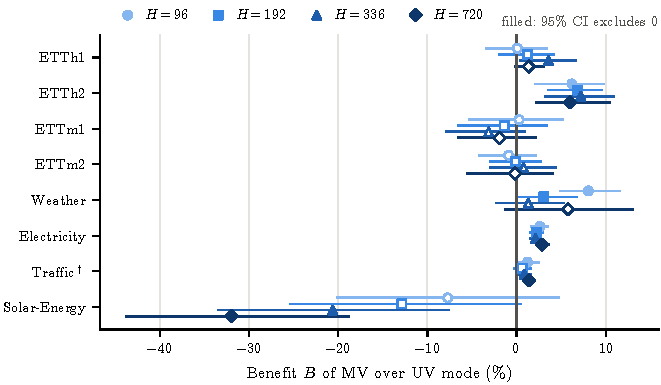
\includegraphics[width=\textwidth]{figures/fig1_benefit.pdf}
  \caption{Benefit $\Ben$ of the \MV{} over the \UV{} mode with 95\% block
  bootstrap intervals, 300 windows per dataset. Positive values favor the
  \MV{} mode. $^\dagger$Potentially seen in pretraining.}
  \label{fig:benefit}
\end{figure}

\begin{table}[t]
  \centering
  \caption{\tfm{} in \UV{} and \MV{} mode. MSE is averaged over the four
  horizons; $\Ben$ (\%) is given per horizon. \sig: 95\% bootstrap interval
  excludes zero; \textbf{bold}: Holm-adjusted Wilcoxon $p<0.05$. Source:
  \texttt{e1\_ltsf\_sampled.csv}.}
  \label{tab:ltsf}
  \setlength{\tabcolsep}{4.2pt}
  \small
  \begin{tabular}{@{}lrccrrrr@{}}
    \toprule
    & & \multicolumn{2}{c}{Mean MSE} & \multicolumn{4}{c}{$\Ben$ (\%) at horizon $H$} \\
    \cmidrule(lr){3-4}\cmidrule(l){5-8}
    Dataset & $N$ & \UV & \MV & 96 & 192 & 336 & 720 \\
    \midrule
    ETTh1                &   7 & 0.404 & 0.398 & $+0.08$ & $+1.21$ & $+3.56$\sig & $+1.35$ \\
    ETTh2                &   7 & 0.329 & 0.307 & $\mathbf{+6.21}$\sig & $\mathbf{+6.86}$\sig & $\mathbf{+7.20}$\sig & $+5.99$\sig \\
    ETTm1                &   7 & 0.362 & 0.368 & $+0.27$ & $-1.39$ & $-3.13$ & $-1.92$ \\
    ETTm2                &   7 & 0.299 & 0.299 & $-0.90$ & $-0.12$ & $+0.79$ & $-0.18$ \\
    Weather              &  21 & 0.301 & 0.287 & $\mathbf{+8.04}$\sig & $\mathbf{+3.06}$\sig & $+1.30$ & $+5.76$ \\
    Electricity          & 321 & 0.153 & 0.150 & $\mathbf{+2.60}$\sig & $\mathbf{+2.24}$\sig & $\mathbf{+2.13}$\sig & $\mathbf{+2.86}$\sig \\
    Traffic$^\dagger$    & 862 & 0.378 & 0.374 & $+1.22$\sig & $\mathbf{+0.61}$ & $\mathbf{+0.86}$\sig & $\mathbf{+1.40}$\sig \\
    Solar-Energy         & 137 & 0.256 & 0.306 & $-7.72$ & $-12.88$ & $\mathbf{-20.63}$\sig & $\mathbf{-31.95}$\sig \\
    \bottomrule
  \end{tabular}
\end{table}

Figure~\ref{fig:benefit} and Table~\ref{tab:ltsf} show that the effect of
the \MV{} mode depends on the dataset, and within a dataset on the horizon.

\paragraph{Consistent gains.} ETTh2 gains 6.0--7.2\% at every horizon.
Weather gains 8.04\% at $H=96$ (MSE $0.167\to0.153$, Holm-adjusted
$p=5.4\times10^{-10}$) and 3.06\% at $H=192$; at longer horizons the point
estimates stay positive but the intervals include zero. Electricity gains
2.13--2.86\% with narrow intervals at every horizon (e.g.\ $+2.60\%$
\ci{1.61}{3.60} at $H=96$, Holm-adjusted $p=8.5\times10^{-20}$), and the
per-window median gain is also 2.2--2.5\%, so the gain is spread over most
windows. Traffic gains 0.6--1.4\% in MSE, but its MAE and pinball loss change
by less than 0.4\% in either direction, and it may have been seen in
pretraining.

\paragraph{No effect.} On ETTh1, ETTm1 and ETTm2, 11 of the 12 intervals
include zero and none of the Wilcoxon tests is significant. For the
15-minute ETT datasets the point estimates are mostly negative (ETTm1:
$-3.13\%$ at $H=336$), which agrees with the observation of Song et
al.~\cite{song2026cloc} that suppressing channel communication suits the ETT
data.

\paragraph{Horizon-growing loss on Solar-Energy.} The \MV{} mode raises the
error by 7.72\%, 12.88\%, 20.63\% and 31.95\% at the four horizons (MSE
$0.304\to0.401$ at $H=720$, Holm-adjusted $p=1.1\times10^{-12}$). The loss is
driven by a minority of windows: at $H=96$ the median window is 7.64\%
\emph{better} in the \MV{} mode, while the summed error is 7.72\% worse; by
$H=720$ the median window is also worse ($-18.12\%$). Solar-Energy is the
dataset on which the model's use of other channels is most costly, and we
return to it in RQ2 and RQ4.

\paragraph{Answer to RQ1.} The \MV{} mode helps on Weather, ETTh2 and
Electricity, has no detectable effect on ETTh1, ETTm1 and ETTm2, and hurts on
Solar-Energy by an amount that grows with the horizon. The sampling rate does not
predict the sign: Weather and Solar-Energy are both 10-minute data.

% ---------------------------------------------------------------------
\subsection{RQ2: What Does the Gain Rely On?}\label{sec:rq2}

\begin{figure}[t]
  \centering
  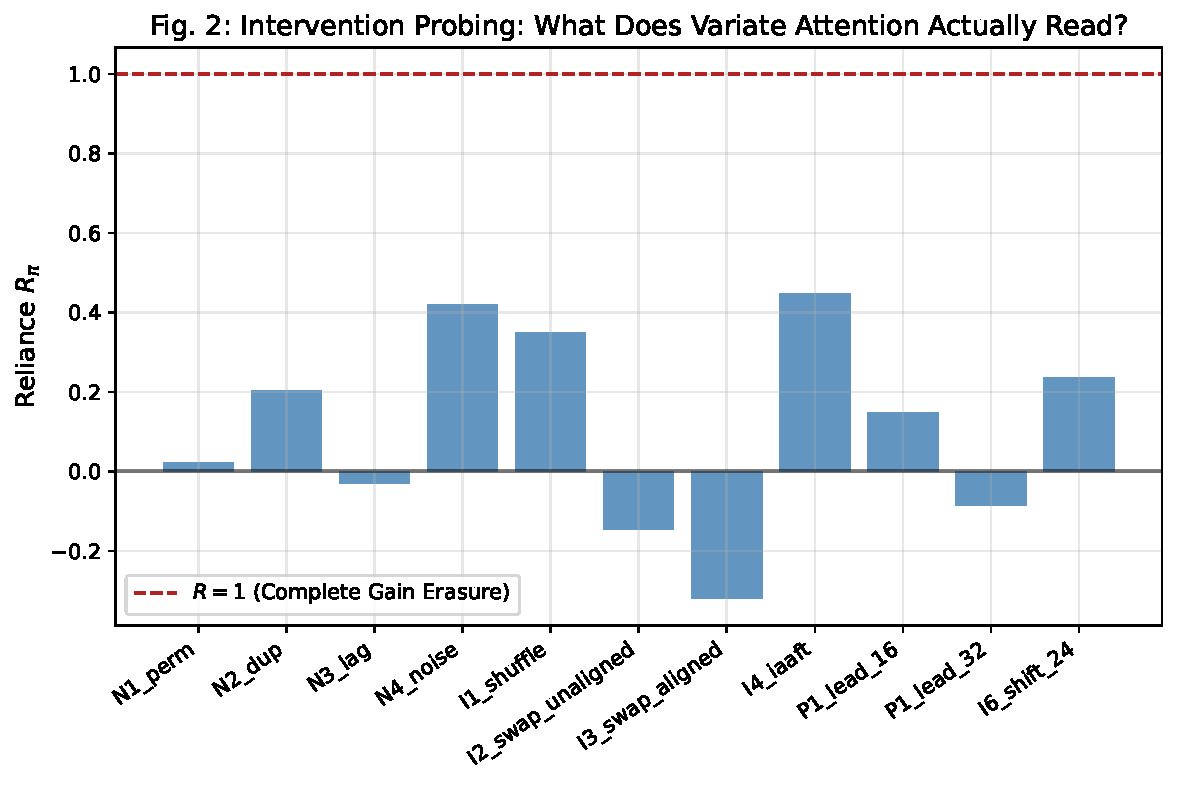
\includegraphics[width=\textwidth]{figures/fig2_interventions.pdf}
  \caption{(a) Reliance $\Rel_\pi$ with 95\% intervals on the two datasets
  whose benefit interval excludes zero at $H=96$. $\Rel=1$: benefit erased;
  $\Rel>1$: worse than the \UV{} mode; arrows mark upper bounds beyond 4.
  (b) Positive control P1: error change relative to the \MV{} mode when a
  noisy copy of the target's future, led by $k$ steps, is added.}
  \label{fig:interventions}
\end{figure}

\begin{table}[t]
  \centering
  \caption{Interventions at $H=96$, 100 windows. For Electricity and Weather
  we report $\Rel_\pi$; for ETTh1 (benefit interval includes zero) and
  Solar-Energy (negative benefit) we report the error change $\Delta_\pi$
  (\%) relative to the \MV{} mode. Brackets: 95\% bootstrap intervals;
  \textbf{bold}: Holm-adjusted $p<0.05$. --: shift exceeds the context.
  Source: \texttt{e2\_interventions\_summary.csv}.}
  \label{tab:e2}
  \setlength{\tabcolsep}{5pt}\renewcommand{\arraystretch}{0.92}
  \scriptsize
  \begin{tabular}{@{}lcccc@{}}
    \toprule
    & \multicolumn{2}{c}{$\Rel_\pi$} & \multicolumn{2}{c}{$\Delta_\pi$ (\%)} \\
    \cmidrule(lr){2-3}\cmidrule(l){4-5}
    & Electricity & Weather & Solar-Energy & ETTh1 \\
    & \vc{$\Ben=+1.61\%$}{0.60}{2.55} & \vc{$\Ben=+12.23\%$}{3.01}{23.04} & \vc{$\Ben=-13.39\%$}{-27.36}{-1.13} & \vc{$\Ben=-0.89\%$}{-5.26}{4.16} \\
    \midrule
    N2 copy      & \vc{$0.03$}{-0.19}{0.18} & \vc{$0.07$}{-0.03}{0.14} & \vc{$-0.07$}{-0.34}{0.19} & \vc{$\mathbf{+0.89}$}{0.26}{1.51} \\
    N3 lag 16    & \vc{$0.11$}{-0.06}{0.42} & \vc{$-0.02$}{-0.23}{0.04} & \vc{$-0.35$}{-1.56}{0.79} & \vc{$+0.93$}{-0.36}{2.14} \\
    N4 noise     & \vc{$\mathbf{1.46}$}{0.89}{3.29} & \vc{$\mathbf{1.63}$}{0.92}{4.66} & \vc{$\mathbf{+11.50}$}{6.31}{17.66} & \vc{$-0.81$}{-3.76}{1.67} \\
    I1 shuffle   & \vc{$\mathbf{1.35}$}{0.86}{2.87} & \vc{$\mathbf{1.00}$}{0.46}{3.28} & \vc{$\mathbf{+13.10}$}{5.75}{21.30} & \vc{$-1.67$}{-4.29}{0.14} \\
    I2 unaligned & \vc{$\mathbf{2.06}$}{1.46}{5.04} & \vc{$\mathbf{0.37}$}{0.14}{1.06} & \vc{$\mathbf{+2.74}$}{-6.84}{13.91} & \vc{$-2.46$}{-5.98}{0.22} \\
    I3 week-aligned & \vc{$0.50$}{-0.31}{1.25} & \vc{$0.89$}{0.32}{3.36} & \vc{$-0.28$}{-12.02}{12.85} & \vc{$-2.27$}{-5.48}{0.23} \\
    I4 IAAFT     & \vc{$\mathbf{1.99}$}{1.39}{4.87} & \vc{$\mathbf{0.66}$}{0.13}{2.06} & \vc{$\mathbf{+38.71}$}{19.38}{65.84} & \vc{$-1.89$}{-4.33}{-0.50} \\
    I5 1 step    & \vc{$0.02$}{-0.15}{0.20} & \vc{$0.04$}{-0.04}{0.19} & \vc{$+0.56$}{-2.21}{2.82} & \vc{$+0.20$}{-0.61}{0.99} \\
    I5 1 h       & (= 1 step)              & \vc{$0.06$}{-0.27}{0.28} & \vc{$\mathbf{+6.23}$}{1.99}{10.90} & (= 1 step) \\
    I5 1 day     & \vc{$\mathbf{1.77}$}{1.17}{4.09} & \vc{$\mathbf{0.98}$}{0.40}{3.18} & \vc{$\mathbf{+56.73}$}{32.73}{90.06} & \vc{$-2.14$}{-4.39}{-0.57} \\
    I5 1 week   & \vc{$\mathbf{1.13}$}{0.69}{2.24} & -- & -- & \vc{$-2.61$}{-5.20}{-0.42} \\
    \midrule
    & \multicolumn{4}{c}{P1 positive control, $\Delta_\pi$ (\%) for all four datasets} \\
    \midrule
    P1 $k=16$    & \vc{$\mathbf{-1.58}$}{-2.37}{-1.06} & \vc{$\mathbf{-9.71}$}{-12.30}{-6.60} & \vc{$-2.11$}{-5.43}{1.10} & \vc{$\mathbf{-10.94}$}{-14.58}{-6.28} \\
    P1 $k=32$    & \vc{$\mathbf{-2.95}$}{-4.19}{-2.14} & \vc{$\mathbf{-18.72}$}{-22.87}{-15.06} & \vc{$\mathbf{-11.12}$}{-17.82}{-4.60} & \vc{$\mathbf{-21.94}$}{-26.00}{-17.01} \\
    P1 6\,h      & \vc{$\mathbf{-0.62}$}{-0.84}{-0.49} & \vc{$\mathbf{-20.58}$}{-24.82}{-16.55} & \vc{$\mathbf{-13.27}$}{-21.97}{-5.17} & \vc{$-3.24$}{-5.32}{-1.27} \\
    \bottomrule
  \end{tabular}
\end{table}

Table~\ref{tab:e2} and Fig.~\ref{fig:interventions} report the interventions.
On Electricity, Weather and Solar-Energy the benefits in this 100-window
sample have the same sign as in RQ1.

\paragraph{Controls.} Permuting the context channels (N1) changes the
forecasts by less than $3\times10^{-7}$ on average on the standardized scale,
which confirms permutation equivariance up to floating-point error. Adding a copy of the target (N2) or a lagged copy
(N3) leaves the benefit unchanged on Electricity and Weather ($|\Rel|\le
0.11$); on ETTh1 the copy raises the error by 0.89\% (Holm-adjusted
$p=0.011$), a small cost of redundant input. The positive control works on all
four datasets (Fig.~\ref{fig:interventions}b): a 32-step leading indicator reduces the error by 21.94\% on
ETTh1, 18.72\% on Weather, 11.12\% on Solar-Energy and 2.95\% on Electricity,
and the reduction grows with the lead. Since a lead of $k$ steps reveals the
first $k$ of the 96 future values, the protocol detects cross-channel use
when the information is present. In a separate diagnostic run on
Solar-Energy with a noise-free 32-step indicator, the error on the first 32
steps fell by 31.83\% \ci{-37.79}{-23.57} (28.48\% with the noise level
of the main run) and on the remaining steps by 9.64\%, so the model uses the
indicator where it is informative. The effect is smallest on Electricity; we
have not identified the cause.

\paragraph{Electricity: calendar-consistent context, not step-level
synchrony.} Shifting the true context by one hour barely matters
($\Rel=0.02$ \ci{-0.15}{0.20}), so the gain does not depend on exact
step-level alignment. What matters is whether the context has the same
calendar phase as the target. Context taken from whole weeks earlier (I3)
keeps about half of the benefit ($\Rel=0.50$), although it is at least 30
days old. Context from 30 days and 7 hours earlier (I2), which differs in
hour and weekday, is worse than no context ($\Rel=2.06$ \ci{1.46}{5.04}); the
two intervals do not overlap. Phase-randomized surrogates that keep each
channel's spectrum (I4, $\Rel=1.99$) and a one-day circular shift that keeps
the hour but not the weekday (I5, $\Rel=1.77$) do the same. These
phase-inconsistent but realistic contexts are at least as harmful as
Gaussian noise ($\Rel=1.46$). The model thus reads the context channels as a
calendar-aligned profile of the current state: when that profile is
consistent with the target, it helps; when it is realistic but out of phase,
the model follows it and the error rises above the \UV{} level.

\paragraph{Weather: recent physical state.} On Weather, shifts of up to one
hour leave the benefit intact ($\Rel\le0.06$), while context that is a day or
more stale, or has lost its temporal order, removes most of it: a one-day
shift ($\Rel=0.98$), week-aligned history ($\Rel=0.89$) and time shuffling
($\Rel=1.00$). Calendar
phase does not rescue the gain here, which fits a weather system with a
diurnal cycle but no weekly one. Noise is the most harmful intervention
($\Rel=1.63$). Unaligned history (I2) keeps part of the benefit
($\Rel=0.37$ \ci{0.14}{1.06}); the interval is wide, and we do not interpret
this value further.

\paragraph{Solar-Energy: close reading, net harm.} Although the \MV{} mode
already hurts on Solar-Energy, the model does not ignore the context: every
information-destroying intervention raises the error further, by 11.50\%
(noise) to 56.73\% (one-day shift), and even a one-hour shift costs 6.23\%.
The forecast moves more than on the other datasets (sensitivity
$\Sen=0.133$ for the one-day shift versus $0.035$ on Electricity). Only a one-step shift, week-aligned history and
unaligned history leave the summed error within its bootstrap interval
($+0.56\%$, $-0.28\%$, $+2.74\%$). Variate attention on Solar-Energy is therefore active and
phase-sensitive, and its net effect is negative.

\paragraph{ETTh1.} Apart from the controls N2 and P1, no intervention is
significant after Holm correction, consistent with the absence of a benefit.

\paragraph{Answer to RQ2.} Where the \MV{} mode helps, the gain depends on
context that is recent (Weather) or calendar-consistent (Electricity); it
tolerates misalignment of up to an hour. Realistic but phase-inconsistent
context is as harmful as noise and pushes the error above the \UV{} level.

% ---------------------------------------------------------------------
\subsection{RQ3: How Much Available Information Is Extracted?}\label{sec:rq3}

\begin{figure}[t]
  \centering
  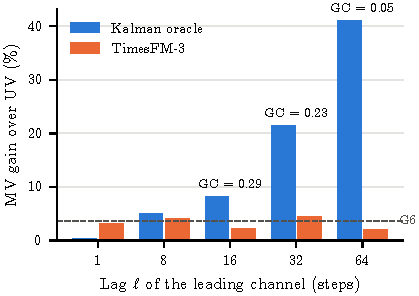
\includegraphics[width=0.62\textwidth]{figures/fig3_leadlag.pdf}
  \caption{Lead--lag generator G5 ($N=8$): improvement of the \MV{} over the
  \UV{} Kalman oracle (available information) and benefit $\Ben$ of \tfm{}.
  Gap closure $\GC$ is shown where the oracle gap is at least 5\%. Dashed:
  benefit of \tfm{} on independent channels (G6). Source:
  \texttt{e3\_synthetic\_summary.csv}.}
  \label{fig:leadlag}
\end{figure}

Figure~\ref{fig:leadlag} shows the lead--lag generator G5. The information
available to an ideal forecaster grows with the lag, from a 0.45\% oracle
improvement at $\ell=1$ to 8.14\%, 21.48\% and 41.10\% at $\ell=16$, 32 and
64. The benefit of \tfm{} does not follow: it stays between 2.09\% and 4.56\%
for every lag. Gap closure therefore falls from 0.29 at $\ell=16$ to 0.23 at
$\ell=32$ and 0.05 at $\ell=64$. At $\ell=1$ the model gains 3.18\%, more
than the 0.45\% the oracle can obtain from the other channels.

The null generator G6 explains this excess. With independent channels, where
the oracle gains nothing, \tfm{} still gains 3.63\% ($N=8$) and 3.13\%
($N=32$). A benefit of about 3\% thus arises without any cross-channel
information, and the lead--lag benefits of 2.1--4.6\% are of the same
size. The model does not exploit a synthetic leading driver, even though it
exploits the leading indicator of P1. The two differ in form: P1 is a shifted
copy of the target, which the model can match by shape, whereas the G5
driver enters the target through its own dynamics and noise. We read this as
evidence that the model follows near-copies in the context better than it
infers a lagged regression, a hypothesis that deserves a direct test.

For the factor (G1), block (G2) and drift (G3) generators the oracle gap was
below 2.4\% in all 33 configurations, and in 11 of them the multivariate
oracle error exceeded the univariate one on the finite test set; these systems
carry too little cross-channel information at our sample size to compute
$\GC$. The model's benefit on them (median 2.66\%, range $-5.15\%$ to
$+6.23\%$) is of the same size as on G6. We did not record bootstrap
intervals for the synthetic runs, so differences of one or two points between
these values should not be interpreted.

\paragraph{Answer to RQ3.} On synthetic data, \tfm{} realizes at most 29\% of
the available lead--lag information and a gain of about 3\% that does not
require cross-channel information. A positive $\Ben$ is therefore not
sufficient evidence of cross-channel use; the interventions of RQ2 are needed
to establish what the gain relies on.

% ---------------------------------------------------------------------
\subsection{RQ4: How Many Channels, and at What Cost?}\label{sec:rq4}

\begin{figure}[t]
  \centering
  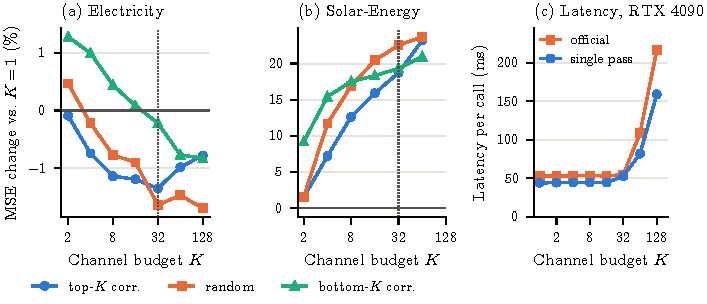
\includegraphics[width=\textwidth]{figures/fig4_budget.pdf}
  \caption{Channel budget $K$ at $H=96$. (a,b) Error change relative to the
  \UV{} mode ($K=1$) when the target is forecast together with the $K-1$
  channels of highest, lowest or random training correlation, in one forward
  pass. (c) Median latency per call on an RTX 4090 for the reference evaluator
  (blocks of 32) and for a single pass over all $K$ channels. Sources:
  \texttt{e5\_grouping\_summary.csv}, \texttt{e5\_official\_chunked\_from\_log.csv}.}
  \label{fig:budget}
\end{figure}

For each target we select $K-1$ companions by absolute training correlation
(top-$K$, bottom-$K$) or at random, and forecast the target together with
them. We run two variants: the reference evaluator, which splits $K>32$
channels into blocks of 32, and a single forward pass over all $K$ channels.

\paragraph{The reference evaluator isolates blocks.} With the reference
evaluator, the error for $K=64$ and $K=128$ is identical to
$K=32$ for every strategy on both datasets (e.g.\ Electricity, top-$K$: MSE
0.1344 at $K=32,64,128$). Channels outside the target's block cannot reach
it, yet each extra block is a sequential forward pass: median latency rises
from 54.8\,ms at $K=32$ to 108.9\,ms at $K=64$ and 217.1\,ms at $K=128$, while
peak memory stays at 1.35\,GB (Fig.~\ref{fig:budget}c).

\paragraph{Accuracy in a single pass.} Removing the cap lets all $K$ channels
interact. On Electricity the error decreases up to $K=32$ and then flattens
(Fig.~\ref{fig:budget}a): random companions give $-1.64\%$ at $K=32$ and
$-1.69\%$ at $K=128$, top-$K$ companions $-1.35\%$ and $-0.78\%$.
The most correlated companions are better than random ones for $K\le16$ (by
0.3--0.6 points) but not for $K\ge32$, where random companions give the
lowest error; the least correlated companions are worst for $K\le64$ (e.g.\
$+1.28\%$ at $K=2$). On Solar-Energy every additional channel raises the
error (Fig.~\ref{fig:budget}b): $+1.51\%$ at $K=2$, $+18.72\%$ at $K=32$ and
$+23.20\%$ at $K=64$ with top-$K$ selection. Top-$K$ selection slows the
degradation at small $K$ ($+12.64\%$ vs.\ $+16.89\%$ random at $K=8$) but
does not reverse it. These differences come from 50 windows and are
small relative to the between-window spread; we treat the ordering of
strategies as indicative.

\paragraph{Cost in a single pass.} Latency stays at 44.2--44.7\,ms for
$K\le16$, so small groups cost no more than the \UV{} mode on this GPU. It
then grows roughly linearly: 52.9\,ms at $K=32$, 82.1\,ms at $K=64$ and
159.2\,ms at $K=128$, with peak memory rising from 1.27 to 1.59\,GB. At
$K=128$ the single pass is 27\% faster than the blocked evaluator and, unlike
it, lets every channel reach the target. The two runs drew their windows and targets
separately and were made at different times, so we compare them only in
latency, and absolute values differ by a few milliseconds.

\paragraph{Answer to RQ4.} Under the reference evaluator, supplying more than
the target's block of 32 channels only adds latency. With a single pass,
Electricity saturates at about 32 channels and gains little from
correlation-based selection at that size, while Solar-Energy is best served
by the \UV{} mode.

% =====================================================================
\section{Data Engineering Guidelines}\label{sec:guidelines}

\paragraph{G1: Decide the mode per dataset and horizon on validation data.}
The benefit ranged from $-31.95\%$ to $+8.04\%$ across datasets and changed
with the horizon within a dataset (Weather: $+8.04\%$ at $H=96$, interval
including zero at $H=336$). A paired \UV/\MV{} comparison on a validation
split costs two inference runs and should precede deployment. Zero-inflated
series with sharp daily transitions, such as Solar-Energy, should default to
the \UV{} mode.

\paragraph{G2: Verify what a gain relies on before trusting it.} Because a
benefit of about 3\% appears on independent synthetic channels, a positive
validation benefit does not show that the model reads useful cross-channel
information. Two cheap checks separate the cases: a one-hour shift of the
context (which should leave the benefit intact) and a one-day shift (which
should remove it if the context matters).

\paragraph{G3: Align timestamps to within an hour and drop stale channels.}
The gain tolerated one hour of misalignment but turned into a loss when the
context was a day stale or out of calendar phase ($\Rel$ up to 2.06). In a
pipeline that joins sensor feeds, late-arriving feeds that would be
forward-filled or joined with a day's delay should be excluded rather than
passed to the model, and clock offsets should be corrected before the join.

\paragraph{G4: Filter noisy and dead channels.} Noise-like channels removed
the benefit on Electricity and Weather ($\Rel=1.46$, $1.63$) and raised the
error by 11.50\% on Solar-Energy. Channels with failing sensors or constant
values should be removed before inference.

\paragraph{G5: Build the blocks explicitly.} The reference evaluator groups
channels by column order, so the table layout decides which channels
interact, and channels outside the target's block add latency without
effect. Constructing groups of at most 32 channels that contain the target
and its intended companions avoids this cost. On Electricity at $K=32$, random
companions were as good as the most correlated ones, so a correlation
analysis over all channel pairs is not required to form useful groups of
that size.

\paragraph{G6: Budget latency by block size.} On an RTX 4090 a single pass
over up to 16 channels costs the same as a univariate call (44\,ms), and
latency grows about linearly beyond 32 channels. Serving systems can pack up
to 16 channels per request at no extra cost and should expect up to
2$\times$ latency for each doubling of the channel count beyond 32.

\paragraph{G7: Supply leading indicators when they exist.} A channel that
leads the target is exploited (up to 21.94\% lower error), so known leading
signals, such as scheduled load or upstream sensors, are the channels most
worth adding.

% =====================================================================
\section{Related Work}\label{sec:related}

\subsubsection{Multivariate TSFMs.}
Moirai~\cite{woo2024moirai} flattens all variates into one sequence with
learned variate biases, and its successor Moirai 2.0~\cite{liu2025moirai2}
returns to univariate forecasting. Chronos-2~\cite{ansari2025chronos2}
applies group attention across series at each patch position and learns
multivariate behavior from synthetic data. \tfm{}~\cite{timesfm3_blog2026}
and Toto~2.0~\cite{khwaja2026toto2} alternate attention along time with
attention across variates, whereas TiRex-2~\cite{carlsen2026tirex2} lets
targets read covariates asymmetrically. Sun et al.~\cite{rmisc2026} report
that real multivariate pretraining data improve over synthetic
multivariatization. Falcon-X~\cite{liu2026falconx} is the closest work: its
authors observe that Chronos-2 is nearly insensitive to disabling group
attention and use the observation to motivate a new architecture. We instead
turn the question into a controlled probe of \tfm{} and characterize when
variate attention helps, is idle, or hurts.

\subsubsection{Channel independence and dependence.}
Channel-independent models such as PatchTST~\cite{nie2023patchtst} and
DLinear~\cite{zeng2023dlinear} match or exceed channel-dependent
Transformers~\cite{zhou2021informer,wu2021autoformer,zhou2022fedformer};
iTransformer~\cite{liu2024itransformer} treats each variate as a token. Han
et al.~\cite{han2024capacity} explain the advantage of channel independence
by a trade-off between capacity and robustness. Abdelmalak et
al.~\cite{abdelmalak2025lookback} find weak Granger causality in standard
benchmarks: channel-independent models win 21 of 28 comparisons there, while
channel-dependent models win 18 of 24 on coupled ODE systems. Song et
al.~\cite{song2026cloc} regulate local and global channel communication per
dataset and find that suppression suits ETT while Electricity and
Solar-Energy benefit from communication. LIFT~\cite{lift2024} identifies
leading indicators as a main source of cross-channel information, and
CPiRi~\cite{cpiri2026} shows that channel-dependent models can overfit the
channel order. These studies train one model per dataset. We ask the
corresponding questions for a single pretrained model at inference time,
where cross-channel use can be switched off and manipulated without
retraining. Our results differ from the supervised picture in one respect:
Song et al.~\cite{song2026cloc} find communication useful on Solar-Energy,
where \tfm{} is harmed by it.

\subsubsection{Evaluating and probing TSFMs.}
GIFT-Eval~\cite{gifteval2024}, fev-bench~\cite{fevbench2025} and
TIME~\cite{timebench2026} compare models across many tasks; such comparisons
confound cross-channel attention with all other differences between models.
We intervene on inputs rather than
inspect attention maps~\cite{jain2019attention} and use IAAFT
surrogates~\cite{schreiber1996surrogate}, a standard tool for destroying
phase relations while keeping each channel's spectrum and marginal
distribution.

% =====================================================================
\section{Conclusion}\label{sec:conclusion}

We probed the variate attention of \tfm{} with paired mode switches,
controlled interventions and synthetic oracles. The \MV{} mode pays off on
Weather, ETTh2 and Electricity, is idle on three ETT datasets and hurts on
Solar-Energy by up to 31.95\%. Where it helps, the gain rests on recent or
calendar-consistent context and tolerates an hour of misalignment;
realistic but out-of-phase context is as harmful as noise. An injected
leading indicator is used, a synthetic lead--lag driver is not, and about
3\% of benefit appears without any cross-channel information. The reference
evaluator's 32-variate blocks make channels beyond the target's block cost
latency without effect.

\paragraph{Limitations.} We study one model; the protocol applies unchanged
to Chronos-2, Toto~2.0 and TiRex-2, and repeating it on these models is the
next step. We did not compare against supervised channel-dependent
baselines. The interventions use a single horizon ($H=96$) and 100 windows,
the synthetic runs lack confidence intervals, and the G1--G3 generators
produced oracle gaps too small for gap closure. Traffic may have been seen
in pretraining. Code, configurations and raw outputs will be released at
\url{https://anonymous.4open.science} upon acceptance.

\bibliographystyle{splncs04}
\bibliography{references}

\end{document}
